\documentclass[12pt]{article}
\usepackage[a4paper, left=2cm, right=2cm, top=2cm, bottom=2cm]{geometry}
\usepackage[utf8]{inputenc}
\usepackage[T1]{fontenc}
\usepackage[french]{babel}
\usepackage{graphicx}
\usepackage{lmodern}
\usepackage{csquotes}
\usepackage[backend=biber,style=numeric,sorting=none]{biblatex}
\usepackage[xindy]{glossaries}
\usepackage[hidelinks]{hyperref}
%\graphicspath{ {images/} }
 
\parskip=5pt plus2pt minus 1pt
\frenchbsetup{ReduceListSpacing=false}

\catcode`\|=13
\def|#1|{\texttt{\detokenize{#1}}}

\addbibresource{bibli.bib}
\makeglossaries

\title{\gls{PdP} \smallbreak Développement d'un moteur de rendu 2D en Rust et OpenGL 4}
\author{Lorian Corbel \\ Camille Meyrignac \\ Maxime Pacaud \\ Nicolas Sentout}

\begin{document}

% ACRONYMS HERE
\newacronym{PdP}{PdP}{Projet de Programmation}
\newacronym{GPU}{GPU}{Graphics Processing Unit}
\newacronym{GLSL}{GLSL}{OpenGL Shading Language}
\newacronym{VBO}{VBO}{Vertex Buffer Object}
\newacronym{IBO}{IBO}{Index Buffer Object}
\newacronym{VAO}{VAO}{Vertex Array Object}

% DEFINITIONS HERE
\newglossaryentry{marque}
{ 
    name=marque,  
    description={Les marques sont les éléments basiques, c'est à dire des formes primitives dont les
    propriétés peuvent être gérées par des données liées} 
}
\newglossaryentry{canaux}
{ 
    name=canaux,  
    description={Caractéristique d'une marque; ex: position, taille, rotation, profondeur, couleur, etc} 
}
\newglossaryentry{crate}
{
    name=crate,  
    description={Une crate est une collection de code source Rust} 
}
\newglossaryentry{shader}
{
    name=shader,
    description={Programme GLSL}
}
\newglossaryentry{vertex}
{
    name=vertex,
    description={Point d'informations graphiques}
}
\newglossaryentry{uniform}
{
    name=uniform,
    description={Un uniform est une variable globale GLSL}
}
\newglossaryentry{pipeline}
{
    name=pipeline,
    description={Succession des opérations généralement réalisées par une carte graphique nécessaires au
    rendu d'un lot de données}
}
\newglossaryentry{geom}
{
    name={geometry shader},
    description={Un programme shader écrit en GLSL qui régit le traitement des primitives (marque)}
}

\maketitle
\tableofcontents
\newpage

\section{Introduction}
Ce projet consiste à développer un moteur de rendu de marques 2D, supportant des animations, le but
principal étant d'avoir une bibliothèque performante, capable d'afficher un grand nombre de marques de
manière fluide.
Pour cela le langage Rust\cite{rust} sera utilisé pour la manipulation des données, ce choix se justifiant
par les garanties de sécurité avec notamment une garantie d'absence d'erreur de segmentation que ce langage
permet mais aussi en étant assez bas niveau pour permettre des performances comparable à un programme
bien sécurisé écrit en C++. De plus l'\gls{GLSL} est utilisé du fait de son contrôle avancé du pipeline du
\gls{GPU}, ce qui est cohérent avec la recherche de performance demandée. Le but final recherché
est d'alléger la charge du CPU. C'est pour cette raison que le
GPU doit être mis à contribution pour tracer les marques à l'aide essentiellement de
\gls{geom}s. C'est-à-dire que les points composant les marques doivent être
majoritairement extrapolés.
 
A partir de maintenant, nous nous référerons à cette bibliothèque par le nom de \og contrast \fg{}.

\section{Description et analyse de l’existant}
Comme expliqué dans l'article introduisant FATuM\cite{FATuM}, la visualisation de l'information est un
domaine très étudié, de ce fait il existe une multitude de système créée pour résoudre ce problème, dont un
certain nombre de bibliothèques qui peuvent être séparées en deux types : les bibliothèques de haut niveau
et celles de bas niveau. Dans notre cas, seules les bibliothèques de bas niveaux nous intéressent quand il
s'agit d'étudier l'existant.
Malheureusement, ces bibliothèques de bas niveau manquent d'abstraction, du fait qu'elles aient été conçues
pour être efficace pour dessiner des primitives mais il n'est donc pas très aisé de les utiliser pour la
visualisation de données et d'un autre côté, les bibliothèques de haut niveau sont peu efficaces et ne
peuvent donc pas gérer de nombreux éléments à la fois.

Il existe aussi l'implémentation de FATuM en C++/OpenGL\cite{LearnOpenGL}, implémenté par les auteurs de
l'article introduisant FATuM. Cette bibliothèque est très efficace avec notamment un benchmark montrant son
efficacité avec un affichage de 200 000 éléments à 60 images par seconde sur une fenêtre de résolution
800x800, sur un ordinateur portable haut de gamme (Intel Core i7-4710HQ CPU@2.50GHz et une carte graphique
Nvidia GeForce GTX 970M).

Il y a aussi le prototype de Romain Giot, programmé en Rust, utilisant luminance\cite{Luminance} et
GLSL\cite{GLSL}, montrant la possibilité d'affichage de différentes marques.

\section{Analyse des besoins fonctionnels}

L'utilisateur doit être capable d'appeler des fonctions de la bibliothèque permettant d'afficher des
\gls{marque}s \cite{VegaMarks}. Il doit notamment être capable de préciser des \gls{canaux} associés à
ces marques : la position de la marque, sa taille, sa rotation, sa profondeur, sa couleur, sa forme,
l'épaisseur et la couleur de son contour, son contraste, sa luminance, son rayon, ses angles, etc.
\textit{Contrast} offrira la possibilité d'afficher les marques suivantes : 
\begin{itemize}
    \item Points : utilisable pour faire des nuages de points. La forme des points dépend d'une fonction de
    distance calculée en GLSL. Les marques de type Points peuvent prendre différentes formes (triangle, rectangle, diamant, trèfle, astérisque, etc.).
    \item Lignes : utilisable tel quel ou pour faire des connexions entre d'autres marques. Les lignes
    peuvent être des segments, des polylignes ou des courbes, elles peuvent aussi avoir différents types
    (continu, tirets, pointillés...).
    \item Polygones : utilisable pour représenter des polygones pleins ou vides, où l'on appelle vide un 
    polygone dont seulement les contours sont dessinés, la couleur de remplissage du polygone plein peut être
    différente de la couleur des contours.
    \item Aires : utilisable pour représenter des polygones ayant un mode d'affichage légèrement différent
    \cite{VegaMarks}.
    \item Texte : utilisable pour représenter du texte et peut avoir différentes propriétés : italique,
    gras, centré, aligné à droite, en haut, etc.
\end{itemize}
    
Pour tester cette fonctionnalité, il devra y avoir des tests permettant d'afficher des marques de façon
contrôlée et de ce fait vérifier si les marques s'affichent bien suivant leurs \gls{canaux} associés.

\textit{Contrast} devra également être capable de gérer des calques, c'est-à-dire que l'utilisateur pourra
décider de placer une marque sur un certain calque et une autre marque sur un différent calque. Si ces
marques ont la même position, l'une des deux marques cachera la seconde. Cet exemple utilise deux calques
mais il peut y en avoir autant que l'utilisateur le souhaite.

Une caméra simple pour visualiser la scène en 2D doit être implémentée. À priori, elle ne fait pas
de translation, le seul paramètre qu'elle prend en compte est un niveau de zoom ainsi que la taille
de la fenêtre d'affichage.

Ces marques pourront également être animées. La gestion des animations sera implémentée de manière similaire
à FATuM, c'est-à-dire avec un double tampon pour la visualisation, un tampon servant de tampon avant et un tampon servant de tampon arrière. Le tampon avant est utilisé pour l'affichage et le tampon arrière est utilisé pour les modifications de l'image affichée et quand l'opération de mise à jour est finie (c'est-à-dire que l'on a une autre image à afficher). Les deux tampons peuvent être échangés par différentes techniques notamment un simple échange : le tampon arrière devient le tampon avant et inversement, ou on peut utiliser une interpolation progressive des deux images stockées dans les tampons. De ce fait, l'image affichée n'est changée que quand il y a une autre image prête, ce qui évite le problème de l'affichage se mettant à jour petit à petit, donnant lieu à des animations peu lisible. Un troisième tampon peut être utilisé pour empêcher l'annulation d'une animation si l'utilisateur demande une modification pendant une animation. Le troisième tampon stocke les modifications faites par l'utilisateur durant l'animation et seront utilisées pour la prochaine animation.

Dans un premier temps la bibliothèque ainsi développée devra être capable d'afficher,
à 50 images par seconde, au moins 10 fois plus d’éléments que la librairie JavaScript D3.js. 
Le but final étant que \textit{contrast} ait de meilleures performances que FATuM.

\section{Analyse des besoins non fonctionnels}

Selon le client, il serait préférable d'implémenter les marques dans l'ordre suivant :
\begin{itemize}
    \item Points
    \item Lignes
    \item Polygones
    \item Aires
    \item Texte
\end{itemize}

Concernant l'API de \textit{contrast}, l'utilisateur n'aura pas accès aux
couches inférieures à la bibliothèque. Il n'aura pas accès aux types des marques,
il décrira seulement les propriétés de la marque et \textit{contrast} déterminera
s'il s'agit d'une marque de type point, ligne, texte, etc.
Voici un exemple de syntaxe pour ajouter une marque de type Texte :

|addMark().set_center(0.5,0.5).set_color(Color.Blue)|\newline
|.set_font("ComicSansMS").set_font_size(20).text("Bonjour").show()|

Notons que cette syntaxe n'est pas définitive mais cela donne une idée de la façon
dont l'utilisateur manipule les marques.

Notre client souhaite que nous utilisons une crate Rust pour compiler
nos shaders en GLSL, afin de construire et nous assurer de leur bonne conformité.
La crate en question porte le même nom que GLSL\cite{GLSL}.

Pour atteindre les demandes de performances imposées par le client, nous allouerons les données au maximum possible sur la pile.
La consommation mémoire n'est pas une contrainte importante pour le développement de \textit{contrast}. Tant
que la vitesse est satisfaisante, nous n'aurons pas à optimiser au mieux la gestion de la mémoire.

Nous devrons mettre en place une batterie de tests importants car ce genre de bibliothèque impose de faire
du code \og non stable \fg{}.
C'est-à-dire du code qui désactive les garanties de sécurité comme celle citée dans l'introduction.
Ces tests permettront en outre de valider nos structures de données.
Nous allons également réaliser des tests de performance afin de nous assurer que notre solution réponde bien
aux exigences de vitesse qui nous sont fixés.

\section{Diagramme de l'architecture}

Ce diagramme, disponible ici (figure~\ref{fig:arch}), décrit les structures, énumérations et traits
(interfaces) qui seront utilisés dans le projet. Il n'y a ni classes, ni héritage dans Rust. C'est
pourquoi ce diagramme est différent d'un diagramme de classes classique.

\begin{figure}[htp]
  \centering
  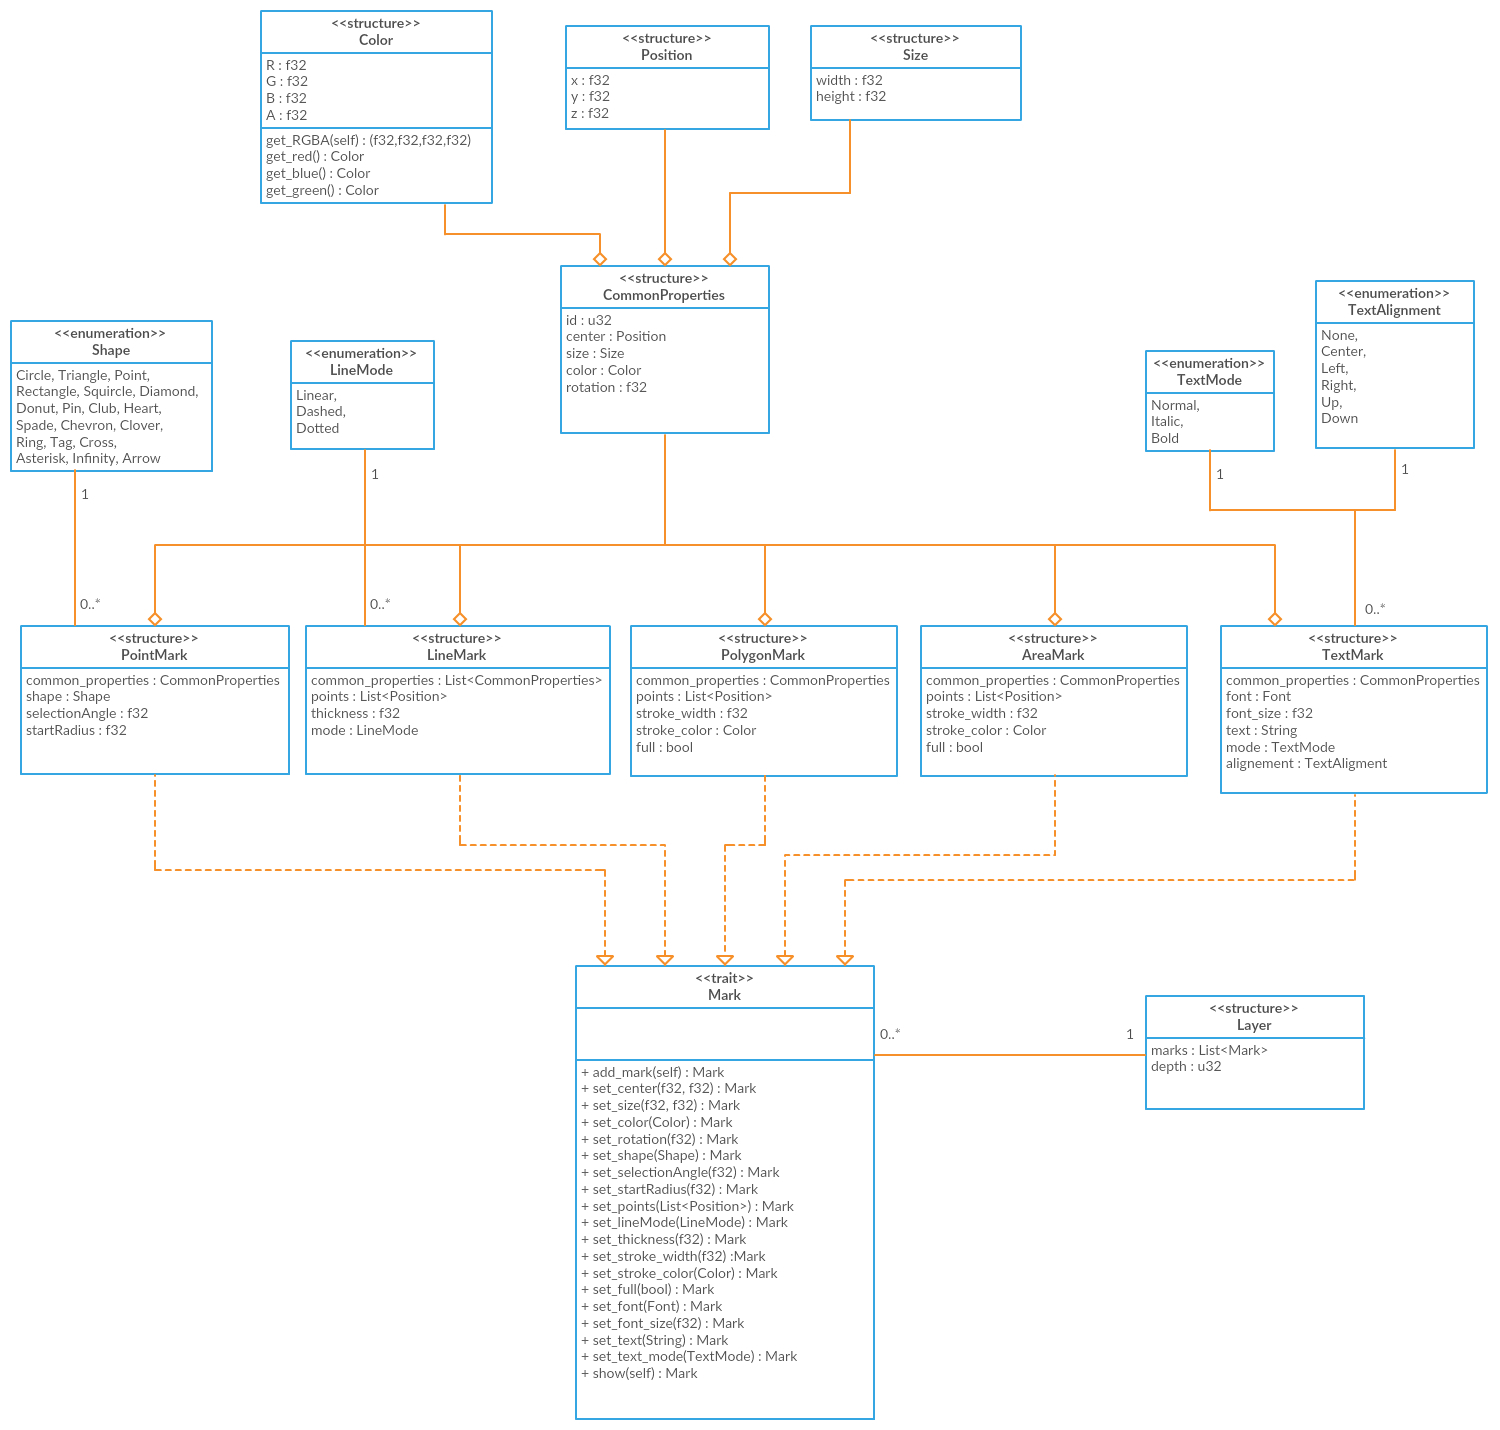
\includegraphics[scale=0.35]{images/architecture}
  \caption{Diagramme de l'architecture de \textit{contrast}}
  \label{fig:arch}
\end{figure}

\section{Schéma du pipeline}

Cette figure~\ref{fig:pipe} présente la décomposition des différents éléments nécessaire au \gls{pipeline}
graphique pour chaque marque. Le pipeline peut être externe à notre bibliothèque, il doit juste demander
les canaux, autrement dit les vertices (\gls{vertex}), contenu dans le \gls{VBO} et les \gls{uniform}
du \gls{shader} à notre bibliothèque\cite{Semi}.
Dans notre cas, c'est \textit{luminance} qui est en charge du pipeline.

Le renderer n'est actuellement pas présent dans notre diagramme de l'architecture pour des 
raisons techniques. Son rôle est d'indexer les marques de chaque type. Quand une marque demande
à être affiché, elle notifie le renderer qui va récupérer ses canaux et construire le VBO.

\begin{figure}[htp]
  \centering
  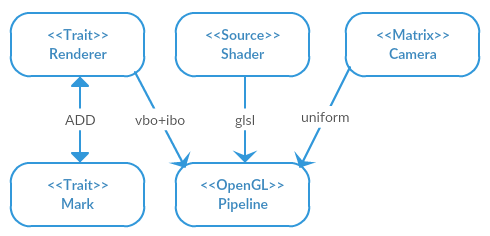
\includegraphics[scale=0.8]{images/pipeline}
  \caption{Diagramme de schématisation du pipeline}
  \label{fig:pipe}
\end{figure}

\section{Diagramme de Gantt}
La figure~\ref{fig:gantt} représente l'organisation de nos différentes tâches en fonction du temps du
projet. 

\begin{figure}[htp]
  \centering
  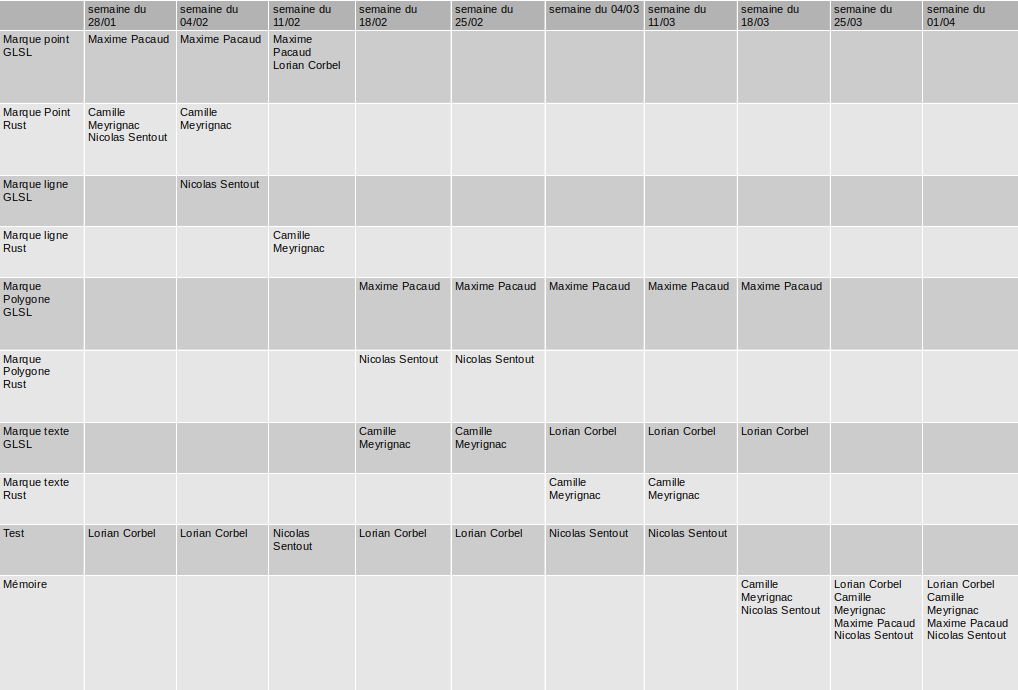
\includegraphics[scale=0.65]{images/gantt}
  \caption{Diagramme de Gantt}
  \label{fig:gantt}
\end{figure}

%\section{Brouillon}
%%%%%%%%%%%%%%%%%%%%%%%%%%%%%%%%%%%%%%%%%%%%%%%%%%%%%%%%%%%%%%%%%%%%%%%%%%%%%%%%
%%%%%%%%%%%%%%%%%%%%%%%%%%%%%%%%%%%%%%%%%%%%%%%%%%%%%%%%%%%%%%%%%%%%%%%%%%%%%%%%
%%%%%%%%%%%%%%%%%%%%%%%%%%%%%%%%%%%%%%%%%%%%%%%%%%%%%%%%%%%%%%%%%%%%%%%%%%%%%%%%
%%%%%%%%%%%%%%%%%%%%%%%%%%%%%%%%%%%%%%%%%%%%%%%%%%%%%%%%%%%%%%%%%%%%%%%%%%%%%%%%
%%%%%%%%%%%%%%%%%%%% A ENLEVER POUR LE RENDU%%%%%%%%%%%%%%%%%%%%%%%%%%%%%%%%%%%%
%%%%%%%%%%%%%%%%%%%%%%%%%%%%%%%%%%%%%%%%%%%%%%%%%%%%%%%%%%%%%%%%%%%%%%%%%%%%%%%%
%%%%%%%%%%%%%%%%%%%%%%%%%%%%%%%%%%%%%%%%%%%%%%%%%%%%%%%%%%%%%%%%%%%%%%%%%%%%%%%%
%%%%%%%%%%%%%%%%%%%%%%%%%%%%%%%%%%%%%%%%%%%%%%%%%%%%%%%%%%%%%%%%%%%%%%%%%%%%%%%%
%%%%%%%%%%%%%%%%%%%%%%%%%%%%%%%%%%%%%%%%%%%%%%%%%%%%%%%%%%%%%%%%%%%%%%%%%%%%%%%%
%\og Bonus \fg{} dont le client nous a parlé :
%\begin{itemize}
%    \item Triple buffer (pour gérer les animations à la FATuM).
%    \item \gls{crate} indépendante (notre librairie ne doit pas dépendre de luminance).
%)\end{itemize}
%

% La bibliothèque ainsi développée servira de support à une bibliothèque de plus haut niveau.

%\nocite{*}
\printglossaries
\printbibliography
 
\end{document}